%\documentclass[twocolumn, amsmath,amssymb, superscriptaddress]{revtex4-2}
%\documentclass[onecolumn, showpacs, preprint,aps,amsmath, amssymb, superscriptaddress]{revtex4}
\documentclass[onecolumn, preprint,aps,amsmath, amssymb, superscriptaddress]{revtex4}

\usepackage{dcolumn}% Align table columns on decimal point
\usepackage{bm}% bold math
\usepackage{amsmath}
\usepackage{amsfonts}
\usepackage{graphics}
\usepackage[dvips]{graphicx}
\usepackage{times}
\usepackage{setspace}
\usepackage{booktabs}

\graphicspath{{figures/}}

\begin{document}

\title{Multifractal detrended cross correlation analysis between Darwin and Tahiti stations}

\author{Sebastián Jaroszewicz}
\author{Cristina Mariani}
\affiliation{Comisi\'on Nacional de Energ\'ia At\'omica, Bs. As., Argentina}
\author{Cristina Mariani}
\affiliation{UTEP, El Paso, United States}
\affiliation{Faculty of Physics, Mathematics and Computer Science, Cracow University of Technology, Krak\'ow, Poland}

\date{\today}

\begin{abstract}

El Niño Southern Oscillation (ENSO) is a phenomenon caused by the interaction between the Pacific Ocean and the Earth's atmosphere that produces impacts at the climatic, economic and social levels. It produces variations in atmospheric pressure at two weather stations located in Darwin and Tahiti, allowing to define the Southern Oscillation Index (SOI). In this article, methods such as DFA, DCCA and its multifractal versions MFDFA and MFDCCA were applied to study the data from these stations with the objective of observing if the time series present multifractal characteristics and its source. This allows obtaining relevant information of the complex system under study. We have observed that the SOI presents a multifractal spectrum and that the major contribution is due to the data from the Tahiti station. This multifractality is due to long-range correlations.

\end{abstract}

\maketitle

\section{Introduction}
\label{sec:Intro}

El Niño, and its counterpart La Niña, are two phases of one phenomenon recurring at irregular intervals of between two and seven years, separated by years of neutral conditions.
Under normal conditions, the warm waters of the western Pacific heat the air, which rises, causes precipitation, and circulates eastward as it reaches the stratosphere. It then descends and moves west, where it accumulates warm water.
 During El Niño episodes, warm waters heat the air above them, in this way the temperature changes produced in the water are coupled with the atmosphere. In this way, the central-eastern region of the Pacific becomes the main engine of an atmospheric circulation pattern called the Walker circulation.
In the presence of an intense source of rising humid air, the surface winds along the equator weaken and sometimes change direction, blowing from west to east, causing warm water to enter the eastern Pacific Ocean, which brings with it increased precipitation in that region.
In contrast, during La Niña, those winds strengthen and warm water moves westward, making the eastern Pacific cooler and drier. Therefore, El Niño represents the warm phase of a cycle of warming and cooling of the surface waters of the Tropical Pacific while La Niña represents the cold phase of the cycle.
This atmospheric response forms the El Niño-Southern Oscillation (ENSO) and represents a phenomenon of great importance that contributes to El Niño maintaining and reinforcing itself.

El Niño has important consequences for weather non only in the tropical Pacific but in many regions of the world. As a consequence, local economies related to ecosystems, fisheries and agriculture are greatly affected in many regions of the globe.

The El Niño phenomenon is closely related to a behaviour of the atmosphera called the Southern Oscillation, discover by Sir Gilbert Walker in 1923 \cite{Walker}. This phenomenon consists of a is a seesaw of atmospheric pressures between the Pacific and Indian Oceans. The strenght of the oscillations is measured by the Southern Oscillation Index (SOI) which is defined as the difference in the monthly Surface air pressure between two meteorological stations one at Darwin, Australia and other at the island of Tahiti. El Ni\~no episodes are associated with negative values of the index, while La Ni\~na episodes are associated with positive values of the SOI.

Several studies reported that the SOI index has multifractal characteristics. Various methods were applied to extract the empirical multifractal properties in metereologicla data sets, for instance, Wavelet Transform, Modulus Maxima (WTMM) [55–57], and the Multifractal Detrended Fluctuation Analysis (MFDFA) [58], Multifractal Detrended Cross Correlation analysis [59], Multifractal Detrending Moving-Average Cross Correlation Analysis [60], Multifractal Cross-Correlation Analysis [61]. Although there are many works that study both the statistical and multifractal properties of the SOI, there is no precedent where the same is done with the values of the time series generated by the Darwin and Tahiti stations. We believe that the study of these series will allow a better understanding of the dynamics of the El Ni~no phenomenon.

This is way the main purpose of this article is to study the cross-correlations between the time series of the surface air pressure measured at the Tahiti and Darwin stations under the fractal framework theory. As far as we know, there are no published works that analyze the cross-correlations between both time series. In this article we analyze the cross-correlations between the Darwin and Tahiti monthly surface air pressure by the means of the MultiFractal Detrended Fluctuation cross-correlation Analysis (MFDFA) method.

The paper is organized as follows: in Section 2 the data used are presented. In Section 3 we describe the methods we use in this article. In section 4 we show and discuss the obtained results. Finally we present conclusions in the last section. 


\section{Data}
\label{sec:Data}

The Southern Oscillation Index (SOI) is one measure of the fluctuations in air pressure occurring between the western and eastern tropical Pacific. Traditionally, this index has been calculated based on the differences in air pressure at sea level between the island of Tahiti and the city of Darwin, Australia. The existence of sustained negative values of the SOI frequently indicate episodes of the El Niño phenomenon. Those negative values are usually accompanied by a sustained warming in the central and eastern tropical Pacific Ocean, a decrease in the strength of the Pacific winds and  a reduction in rainfall in eastern and northern Australia.  On the other hand, positive SOI values are associated with strong winds from the Pacific and a warming of the sea north of Australia, popularly called La Niña. These positive values are generally accompanied by cooling of the waters of the central and eastern tropical Pacific Ocean and an increased probability that eastern and northern Australia will be wetter than normal.

Time series in present study were obtained from the Climatic Research Unit, University of East Anglia. The time period spanning from January 1866 to December 2021. The Data contains the surface air pressure measured at the Tahiti ($17^{\circ}$ 40 S, $149^{\circ}$ 25 W) and Darwin stations  ($12^{\circ}$ 27 S, $130^{\circ}$ 50 E) as well as the SOI index values.
The SOI, Thaity and Darwin time series are plotted as a function of time in Figs. \ref{fig:SOI} and \ref{fig:stations}. 

\begin{figure}
\centering{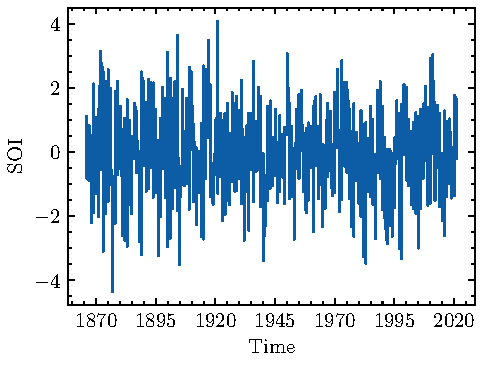
\includegraphics[width=0.42\textwidth]{SOI.pdf}} 
\caption{Monthly values of the SOI from January 1866 to December 2021}
\label{fig:SOI}
\end{figure}

\begin{figure}
\centering{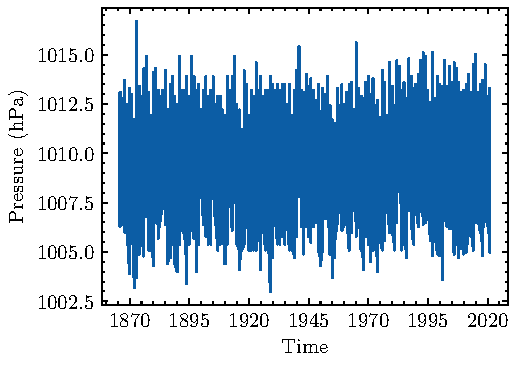
\includegraphics[width=0.42\textwidth]{Darwin.pdf}} 
\centering{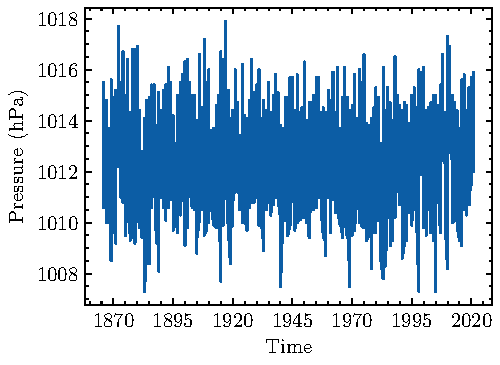
\includegraphics[width=0.38\textwidth]{Tahity.pdf}}
\caption{Manthly values of the sea level preassure in hPa at (a) Darwin station and (b) Tahity station.}
\label{fig:stations}
\end{figure}

We present the descriptive statistics of the indexes used in this study in table \ref{tab:descriptive}. The tables present the mean, minimum, and maximum and the standard deviation of the series, as well as skewness and kurtosis levels.
\begin{table}[]
\caption{Descriptive statistics of studied series.}
\label{tab:descriptive}
\begin{tabular}{lccc}
\hline
          & SOI    & Darwin & Tahity \\ \hline
Mean      & 0.053  & 1010   & 1013   \\
Std. Dev. & 1.28   & 2.65   & 1.71   \\
Minimum   & -4.344 & 1003   & 1007   \\
Maximum   & 4.073  & 1017   & 1018   \\
Skewness  & -0.074 & -0.212 & -0.064 \\
Kurtosis  & 0.217  & -0.948 & -0.200 \\ \hline
\end{tabular}
\end{table}
%All series are negatively skewed, suggesting long left tails. The values of the excess of kurtosis are below minus two for the three series indicating that the indexes are platykurtic.


%There are several slight variations in the SOI values calculated at various centres.

%Here we calculate the SOI based on the method given by Ropelewski and Jones (1987). These authors It uses a second normalization step, and was the Climate Analysis Centre's standard method in 1987. The reader is also referred to Allan et al. (1991) and Können et al. (1998) for details of the early pressure sources and methods used to compile the series from 1866 onwards.

%Main reference to cite when using this SOI index:
%Ropelewski, C.F. and Jones, P.D., 1987: An extension of the Tahiti-Darwin Southern Oscillation Index. Monthly Weather Review 115, 2161-2165.

\section{Methodology}
\label{sec:method}
\subsection{Detendred fluctuation analysis (DFA)}

The detrended fluctuation analysis (DFA) developed by Peng et al. \cite{Peng_3} is an important method  to detect the presence of long-range correlations in time series. By applying DFA, an exponent similar to Hurst is obtained, with the difference that this method can also be applied when the dynamics are not stationary. The DFA has been successfully applied to a wide range of time series in various fields such as  analysis of DNA \cite{Buldyrev_2},\cite{Buldyrev_3}, heart rate dynamics \cite{Peng_2}, \cite{Viswanathan} , \cite{Echeverria}, economical time series \cite{Cizeau}, \cite{Ausloos}, \cite{Jaroszewicz}, \cite{Mariani}, geophysics \cite{Ribeiro}, among others.

We can summarize the DFA procedure in the next three steps

\begin{enumerate}
\item Let $A(k)$ be a possibly non-stationary time series of length $N$. We, first, construct the trajectory or the 'profile' by subtracting from the times series its average and the summing cumulatively.
\begin{equation}
y(k) = \sum_{i=1}^{k}[A(i)-<A>]
\label{profile}
\end{equation} 
\item The profile is sub-divided into $N_s=\text{int}(N/s)$ non-overlapping windows of equal length $s$. Since the length $N$ of the series may not be an integer multiple of the window size $s$, and a short part of the profile $y(k)$ at the end may be disregarded by the procedure, the sub-division is performed also starting from the opposite end, obtaining a total of $2N_S$ segments.

\item In each window $v$ the serie is detrended by substracting the local trend $y_n(k)$, given by a polynomial regression of order $m$,  and the mean square residual $F(v,s)$, for $v=1,\dots,2N_s$, is found as
\begin{equation}
F(v,s) = \sqrt{\dfrac{1}{s}\displaystyle\sum_{i=1}^{s}\left\lbrace y[(v-1)s+i]-y_n[(v-1)s+i]\right\rbrace^2}
\end{equation}
Typically the regression is linear.  
\item The DFA exponent $\alpha$ is the slope of $F(s)$ line in a log-log plot. It can be interpreted as an estimation of the Hurst exponent.
\end{enumerate}

\subsection{Multifractal Detrended Fluctuation Analysis}

As mentioned in the introduction, in this study MFDFA method was applied to study the multifractal characteristics of the analized temporal series. The MFDFA is a well-known technique, and is commonly used to detect multifractality in a time series \cite{Kantelhardt}. \\
The steps of the algorithm are very similar to those described in DFA section where the profile must be constructed, then divide the series into windows and eliminate trends with a fitted polynomial. For each segment $v$, $v=1,\ldots,N_s$  we compute the variance:
\begin{equation}
 	F^2 (s,v)=\frac{1}{s} \sum_{i=1}^s\{y[N-(v-N_s )s+k]-y_n (k)\}^2
 	\label{eq:var2}
\end{equation}

where $v=N_s+1,\ldots,2N_s$. Here $y_v (i)$  is the fitting polynomial in segment $v$. \\
Then, averaging over all segments the $q_{th}$ order fluctuation function is computed

\begin{equation}
F_q (s)=\left\lbrace \frac{1}{2N_s} \sum_{v=1}^{2N_s}[F^2 (s,v)]^{\frac{q}{2}}\right\rbrace ^{1/q}
\label{eq_f}  
\end{equation}

where, in general, the index variable $q$ can take any real value except zero. $F_q (s)$ will increase with increasing $s$ and if $F_q (s)$  behave as a power-law of $s$ the series is scaling for that specific $q$.


\begin{equation}
F_q (s) \propto s^{h_q}.
\end{equation}

The exponent $h_q$ is called generalized Hurst exponent due to the equivalence between $h_2$ and the Hurst exponent ($H$) for stationary series, leading to consider the well know DFA \cite{Peng} a particular case of the MFDFA for $q=2$ \cite{Kantelhardt_2, Zhang}. It can be seen  in Eq.\ref{eq:var2} and Eq.\ref{eq_f}. For $q=0$ the value $h_0$ corresponds to the limit $h_q$ for $q \rightarrow 0$, and is obtained through a logarithmic averaging procedure:

\begin{equation}
F_0(s) \equiv exp \left\lbrace \frac{1}{4N_s} \sum_{v=1}^{2N_s} ln[F^2 (s,v)]\right\rbrace  \propto s^{h_0}.
\end{equation}

For monofractal series $h(q)$ is independent of $q$ because the behavior of $F^2$ in \ref{eq_f} is independent of $q$. On the contrary, for multifractal series the exponent $h_q$ will depend on $q$, and it monotonically decreases with the increase of $q$, the series is multifractal. For positive values of $q$ the function $h(q)$ describes the scaling behavior of the segments with large fluctuations, whereas for negative values of $q$, the scaling behavior of the segments with small fluctuations is described. Based on $h(q)$ the mass exponent $\tau(q)$ (also called R\'enyi exponent) can be calculated as follows

\begin{equation}
\tau(q)=qh_q-1
\label{eq:Reny}
\end{equation}

The application of the Legendre transform to $\tau(q)$ allows us to characterize a multifractal time series through its multifractal spectrum.

\begin{equation}
\alpha=d\tau/dq
\end{equation}

\begin{equation}
f(\alpha)=q\alpha-\tau(q)
\end{equation}

In the above equation $\alpha$ is the H\"older exponent and $f(\alpha)$ is the singularity spectrum that indicates the dimension of the subset of the series that is characterized by $\alpha$. The multifractal spectrum indicates how much dominant are the various fractal exponents present in the series and its width, as well as the range of the generalized Hurst exponent $(max(h_q)-min (h_q))$, are often used to quantitatively measure the degree of multifractality of the series. Thus, the wider the spectrum the more multifractal the series is.

In order to characterize the complexity of the studied process, it is possible to extract a set of parameters from the spectrum. To do this, we adjust the singularity spectrum to a fourth degree polynomial:

\begin{equation}
f(\alpha) =  A + B(\alpha - \alpha_0) + C(\alpha - \alpha_0)^2 + D(\alpha - \alpha_0)^3 + E(\alpha - \alpha_0)^4
\end{equation}

and we calculate the following parameters of the multifractal spectrum: the position of the maximum of the spectrum $\alpha_0$, the width of the spectrum $\omega = \alpha_{max}-\alpha_{min}$, where $\alpha_{max}$ indicates the value of the most extreme events and $\alpha_{min}$that of the softest ones, and, finally, the asymmetry parameter given by $a_s = (\alpha_0-\alpha_{min})/(\alpha_{max}-\alpha_0)$. The parameter $\alpha_0$ provides an estimate of the value of the Hurst exponent, in general a value of $\alpha_0 > 0.5$ indicates a correlated or persistent process, and $\alpha_0 < 0.5$ an anti-correlated or anti-persistent process, while $\alpha_0 = 0.5$ indicates a totally random process. The parameter $\omega$, as indicated above, is the width of the spectrum and measures the amplitude of the fractal exponents necessary to describe the signal. The asymmetry parameter $a_s$ allows us to measure the skewness of $f(\alpha)$, $a_s<1$ indicates a right skewed spectrum while $a_s>1$ a left skewed one. The importance of this parameter resides in that it provides us with information  the prevalence of small and large fluctuations in the multifractal spectrum. If $a_s = 1$, the spectrum is symmetric and both large and small fluctuations contribute equally to multifractality. On the other hand, if the spectrum is asymmetric to the right, the greatest contribution to the multifractal spectrum is given by the subsets with small fluctuations and finally, an asymmetric spectrum to the left indicates that the subsets with large fluctuations are those that contribute the most to the multifractal spectrum.

In summary, these parameters allow us to evaluate the complexity of the process: a time series with a high value of $\alpha_0$, a wide range of fractal exponents, and a right-skewed spectrum can be considered more complex than one with opposite characteristics.

\subsection{DCCA and MF-DCCA}

DCCA was developed by Podobnik et al. \cite{Podobnik} from the well-known DFA method \cite{Peng} with the objective of quantifying the long-term cross-correlation of two non-stationary time series. 

In summary, the method consists of dividing the previously integrated time series $y(k)$ into $N_s$ segments of equal length $s$, and in each of them applying an ordinary linear regression to capture the local trend. 
The integrate series $y_{v,s}(k)$ is then detrended by substracting the local trend from the data in each box and the detrended covariance is calculated as

\begin{equation}
F^2_{DCCA}(v) = \dfrac{1}{vN_s}\sum_{s=0}^{N_s-1}\sum_{k=vs+1}^{v(s+1)}\left[y(k)-y_{v,s+1}(k)\right] \left[y_n(k)-y_{n[v,s+1]}(k)\right]
\end{equation}

The relationship between the length $s$ of the segments and $F_{DCCA}$ is obtained by repeating the calculation for all segments sizes. In case that cross-correlation between series decay as a power law, then the detrending covarianze grows with the time scale as

\begin{equation}
F_{DCCA}\sim s^\lambda
\end{equation}

where $\lambda$ is the DCCA cross-correlation exponent. The value of $\lambda$ can be calculated from a linear regression on a plot of $\log F$ vs $\log \lambda$. If, however, the detrended covariance oscillates around zero as a function of the time scale, there are no long-range cross-correlations.

In order to quantify the information about cross correlations provided by the DCCA, Zebende (2011) built a correlation coefficient that allows to quantify cross-correlation levels across time scales between two different time series ()$X$ and $Y$). This approach combines the DCCA with the detrended fluctuation analysis (DFA). This Detrended cross-correlation coefficient is defined as the ratio between the detrended covariance function $F^2_{DCCA}$ and the detrended variance function \cite{Zebende}
\begin{equation}
    \rho_{DCCA}(s) =\dfrac{F^2_{DCCA(s)}}{F_{DFA_X}F_{DFA_Y}}
\end{equation}
where $F_{DFA_X}$ stands for the DFA method applied to the serie $X$ and $F_{DFA_y}$ for series $Y$ .

DCCA coefficient is a dimensionless quantity and its
values are ranging between $-1 \leq \rho_{DCCA} \leq 1$. If $\rho = 1$, it means that a perfect cross-correlation between series exists, if $\rho = -1$ perfect anticross-correlation exists and there is no cross-correlation between the series if $\rho = 0$. 

MF-DCCA is a generalization of the DCCA introduced by Zhou \cite{Zhou} and differs from MFDFA in that there are now two detrended signals  $\tilde{X}_v(s,i)$ and $\tilde{Y}v(s,i)$ in each window. Therefore, the covariance is defined as

\begin{equation}
F_{XY}^2 (s,v)=\frac{1}{s} \sum_{i=1}^s\tilde{X}_v(s,i)\tilde{Y}_v(s,i)
\end{equation}

Now the $q_{th}$ order fluctuation function is computed by

\begin{equation}
F_q(s) =\left\{ {1 \over  N_s} \sum_{v=1}^{ N_s} \left[ F_{XY}(s,v)
\right]^{q/2} \right\}^{1/q} \label{eq:fdef}
\end{equation}

Generally, $q$ can take any real value, except zero. For $q=0$, equation (\ref{eq:fdef}) becomes:

\begin{equation}
F_0(s)= \exp\left( {1 \over  2N_s} \sum_{v=1}^{ N_s}\ln F_{XY}(s,v)\right
) \label{eq:fdef0}
\end{equation}

For $q=2$, the standard DCCA is retrieved.

In the case that there is a correlation between the two series, we can express the relationship between $F$ and $s$ as

\begin{equation}
F_q(s) \sim s^\lambda(q)
\end{equation}

If $\lambda(q)=0.5$ the two series are not correlated, which means that changes in one do not cause changes in the other. The case $\lambda(q) > 0.5$ indicates the presence of a persistent cross-correlation, which means it is likely that the increase in one series is followed by an increase in the other. Finally if the cross correlation is anti-persistent $\lambda(q) < 0.5$.

Like for the MFDFA if $\lambda(q)$ does not change with $q$, the cross-correlations between the series are monofractal. If $\lambda(q)$ is a decreasing function of $q$ , the cross-correlation between these two time series is multifractal. Like for the MFDFA if the multifractal spectrum ends up being a point, there is no presence of multifractality. A wider multifractal spectrum indicates a stronger degree of multifractality.



\section{Results}
\label{sec:resultados}

\subsection{DFA}
\label{results_dfa}

Firstly we applied the DFA method to the three time series. The size of the analyzed windows ranges from 10 to $N/4$ where $N$ is the length of each series. The double log plot of the fluctuation function for the studied data are shown in Fig. \ref{fig:dfa}. In this figure we can see that the value of scale exponent for large window sizes is well below than 0.5 in the cases of Darwin and SOI indexes suggesting that the series are anti-persistent. This behavior means that an increase in the current period is more likely followed by a decrease in the next period and vice versa. In the case of SOI we can observe a crossover at $\log(s) = 1.7$ that allows us to differentiate between two different scale regimes. The value of the exponent before the crossover reveals a persistent behaviour of the $1/f$ type (pink noise). Interestingly the value of the scale exponent is close to 0.5 for the Tahity case. This fact is more noticeable when several orders of the DFA method are applied. For example for the DFA2 (second order) the value of the exponent is 0.52. Therefore, in the case of Tahity, we cannot ensure that there are long-range correlations. 

\begin{figure}
\centering{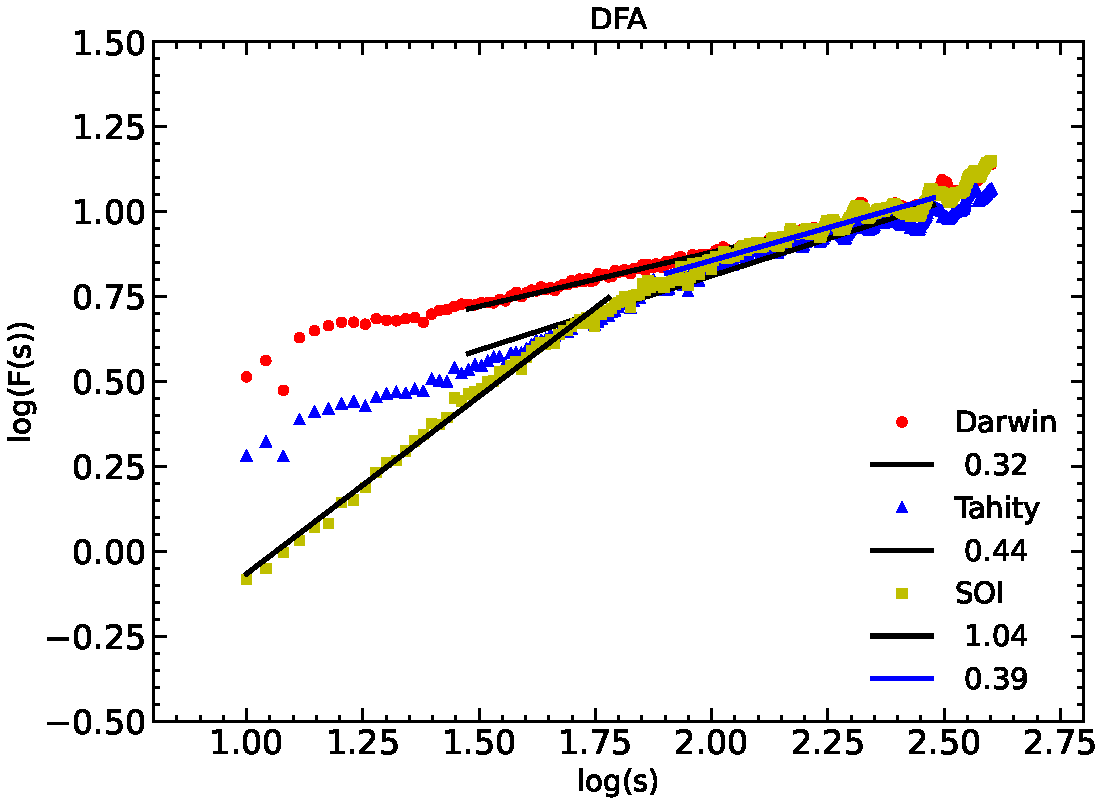
\includegraphics[width=.6\textwidth]{DFA.pdf}} 
\caption{DFA fluctuation function as function of the time scale for the three series.}
\label{fig:dfa}
\end{figure}

\subsection{MFDFA}
\label{results_mfdfa}

The next step was to study the full range of generalized Hurst exponents by means of the MFDFA method. In other words we apply this method to explore the multifractal properties of the series. We applied the MDFA for values of $q$ from $-10$ to $10$ and and in the same temporal range that we used for the DFA. Figs.\ref{fig:mfdfa_dar} to \ref{fig:mfdfa_soi} show the log-log plots of the fluctuation functions for $q=-10,-5,0,5,10$ as examples for each of the series analyzed.

\begin{figure}
\centering{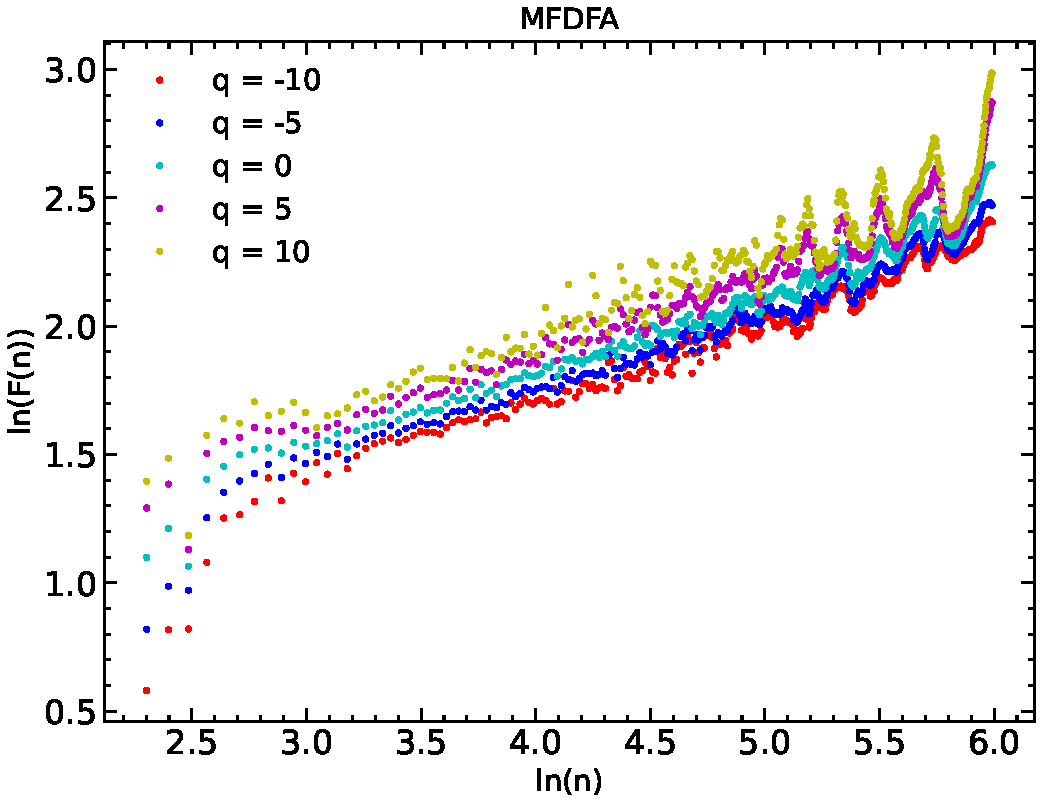
\includegraphics[width=.6\textwidth]{MFDFA_dar.pdf}} 
\caption{Fluctuation functions for Darwin data}
\label{fig:mfdfa_dar}
\end{figure}

\begin{figure}
\centering{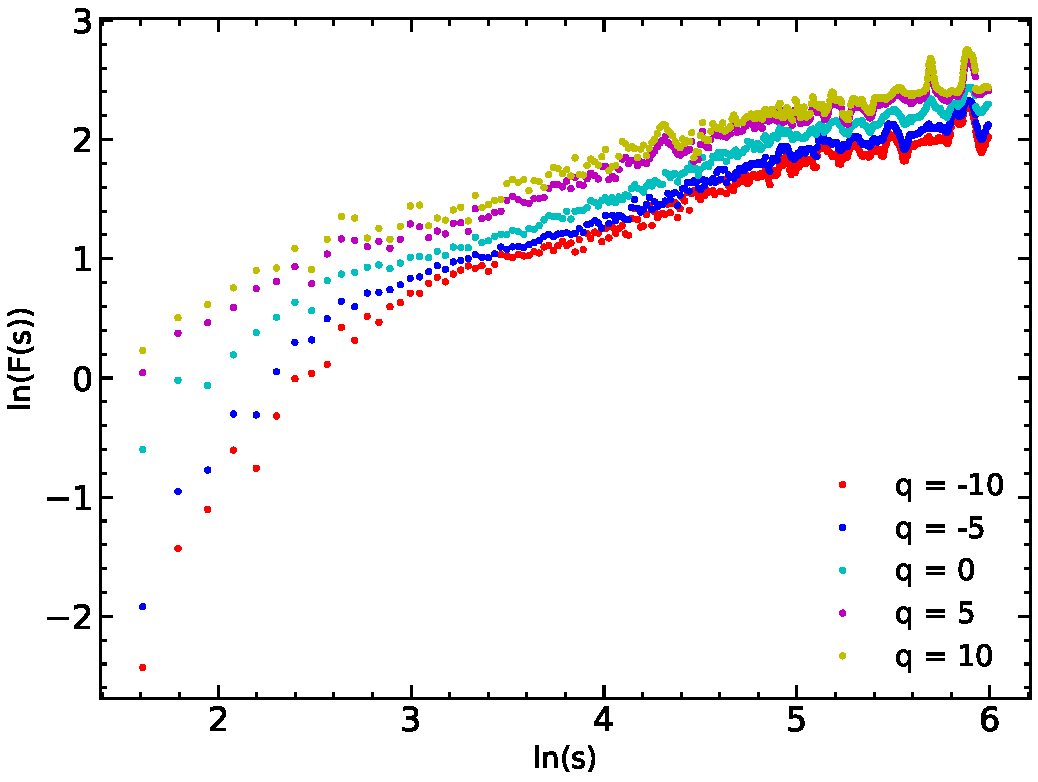
\includegraphics[width=.6\textwidth]{MFDFA_tah.pdf}} 
\caption{Fluctuation functions for Tahity data}
\label{fig:mfdfa_tah}
\end{figure}

\begin{figure}
\centering{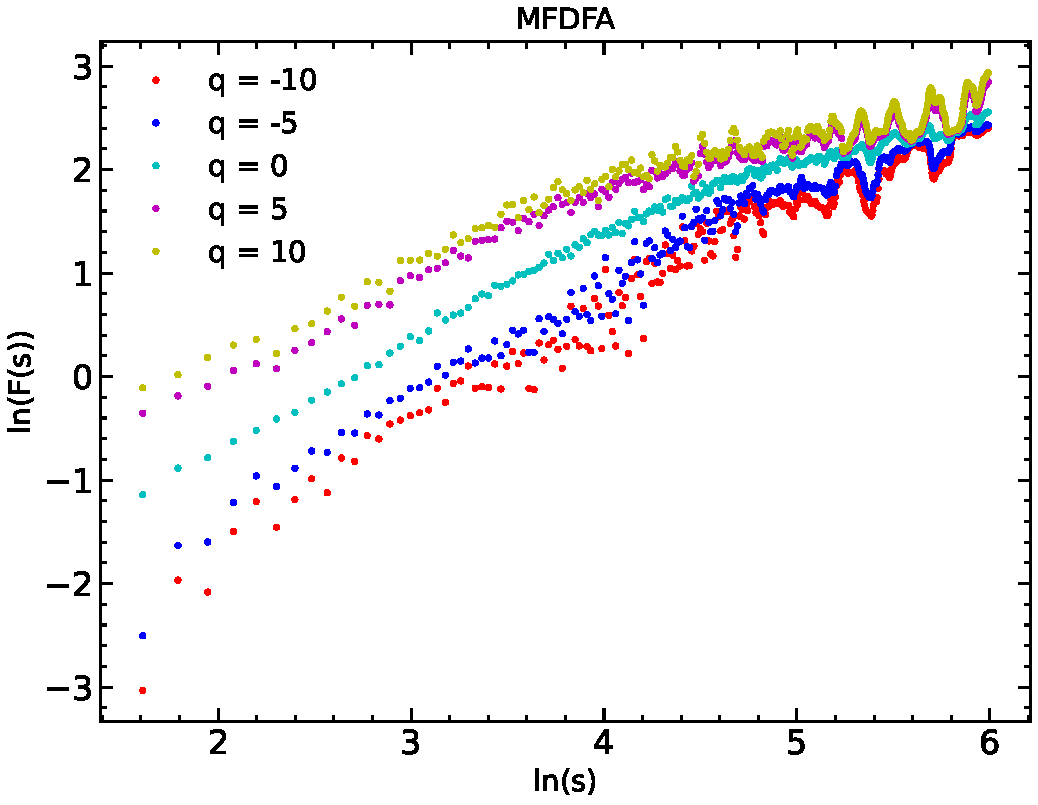
\includegraphics[width=.6\textwidth]{MFDFA_soi.pdf}} 
\caption{Fluctuation functions for SOI data}
\label{fig:mfdfa_soi}
\end{figure}

\begin{table}[t]
\begin{center}
\begin{tabular}{ c  c  c  c  c  c  c  c }
\hline

   & $\alpha_{min}$  & $\alpha_{max}$ & $\alpha_0$ & $f(\alpha_{min})$ & $f(\alpha_{max})$ & $\omega$& $a_s$ \\ \hline
Darwin   & 0.33  & 0.43  & 0.37  & 0.81 &  0.70 &  0.10 &  0.11 \\
Tahity     & 0.35  & 0.61  & 0.49  & 0.45 &  0.52 &  0.26 &  -0.07 \\
SOI     & 0.44  & 1.05  & 0.68  & 0.30 &  0.06 &  0.61 &  0.24 \\
\hline
\end{tabular}
\caption{Characteristics of the multifractal spectrum}
\label{tab:mfdfa}
\end{center}
\end{table}


\begin{figure}
\centering{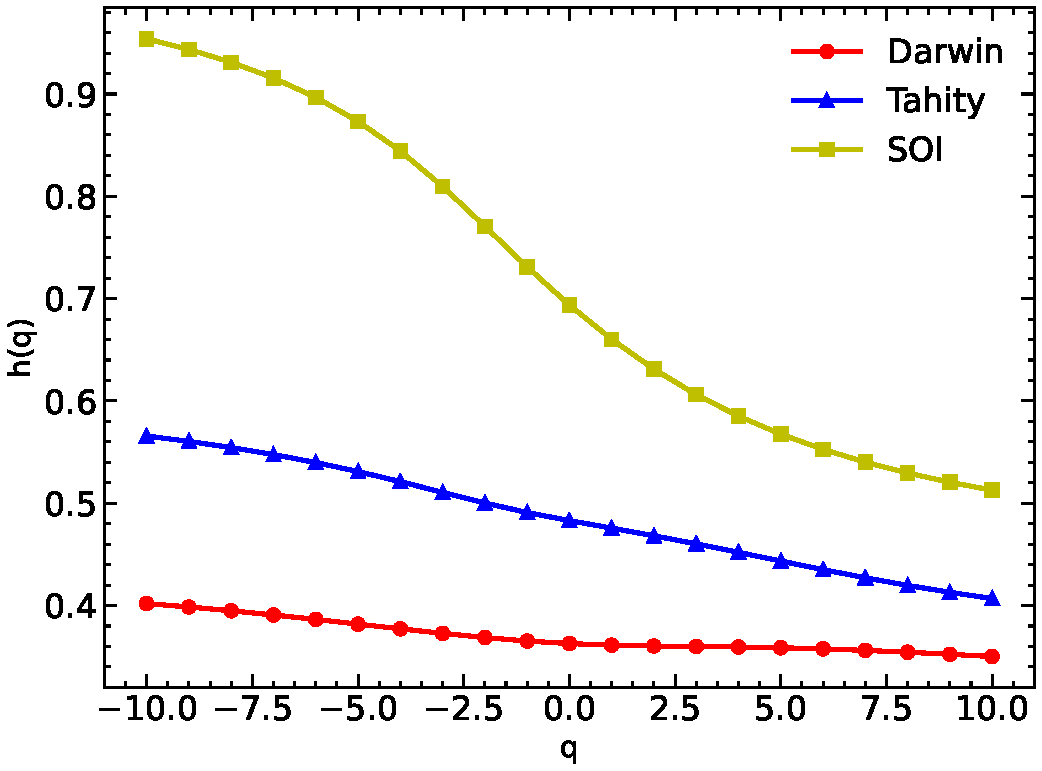
\includegraphics[width=.6\textwidth]{H.pdf}} 
\caption{$q$ dependence of the generalized Hurst exponent}
\label{fig:H}
\end{figure}

\begin{figure}
\centering{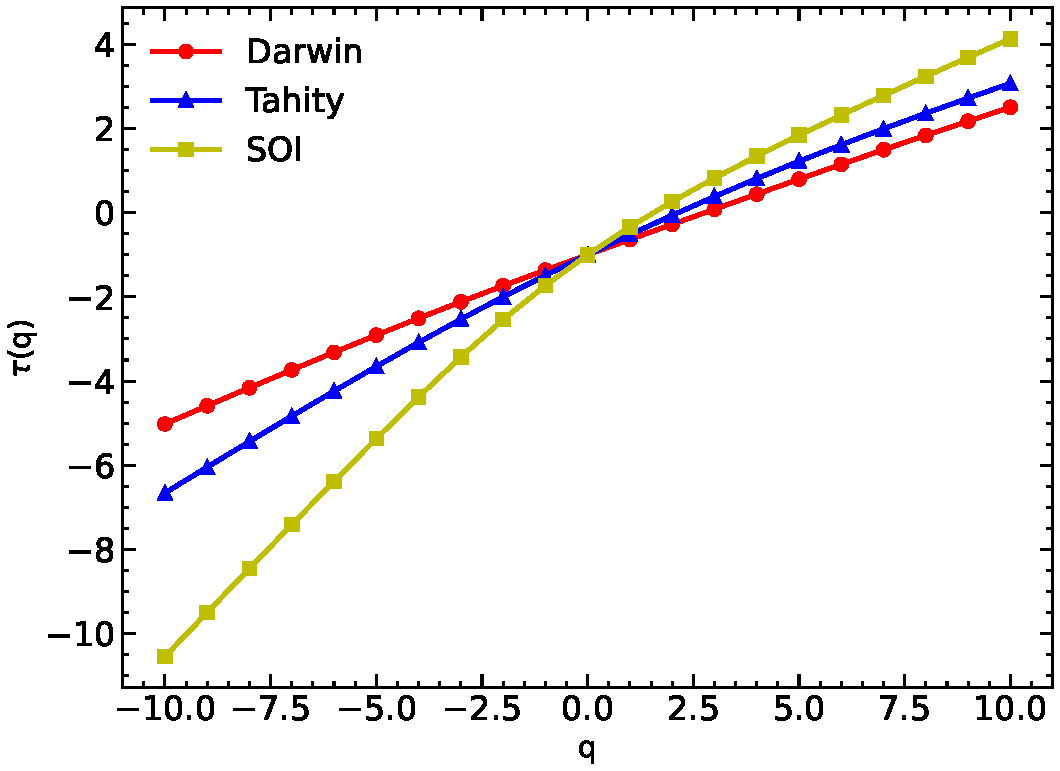
\includegraphics[width=.6\textwidth]{tau.pdf}} 
\caption{Plots of $\tau(q)$ vs $q$}
\label{fig:tau}
\end{figure}

In Fig. \ref{fig:spectrum} the multifractal spectrum for the three series is shown and in Table \ref{tab:mfdfa} the properties of the spectra are summarized. As can be seen both in the table and in the graph, the width of the spectrum $(\omega)$ corresponding to the SOI is much larger than that corresponding to the stations indicating stronger multifractality for the former. Furthermore we can see that the multifractal spectrum corresponding to the series of Darwin and SOI is left-skewed whereas that corresponding to the Tahity series is right-skewed. The left-sided asymmetry that we can observe in the Tahity's spectrum corresponds to a  multifractality on the level of larger fluctuations and its degeneration towards monofractality with fluctuations decreasing. In the case of the other two indices right-sided asymmetry indicates that multifractality is more developed on the level of smaller fluctuations and the larger ones are suppressed.


\begin{figure}
\centering{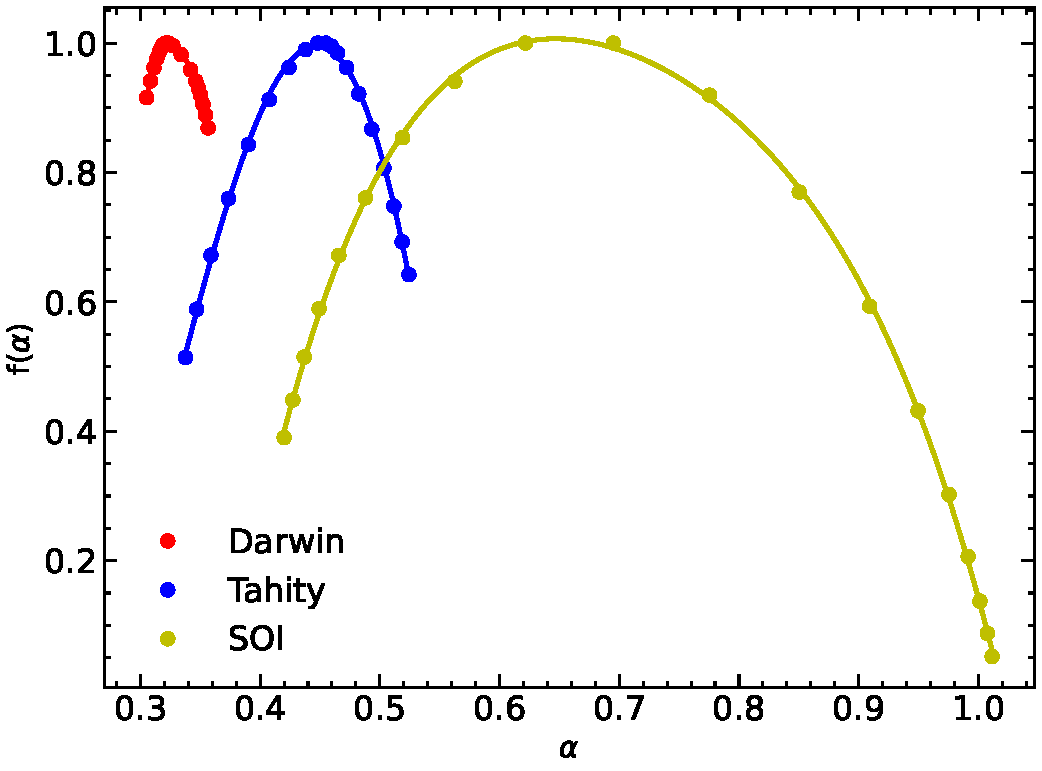
\includegraphics[width=.6\textwidth]{interp_spec.pdf}} 
\caption{Multifractal spectra for the studied series}
\label{fig:spectrum}
\end{figure}



Two sources of multifractality can be recognized: (i) multifractality due to a broad probability density function of the values of the series, and (ii) different long range correlations for small and large fluctuations. To test the type of multifractality one can remove the temporal correlations by random shuffling the series. If the multifractality is of the type stated in the second case the spectrum should be significantly narrowed. Random shuffling simply consists of generating a new time series by randomly permuting the elements of the original series. in order to check if multifractality comes from broad distributions, we analyze surrogate data. To generate them we apply amplitude adjusted fourier transform to the original series. The surrogate time series data did not destroy the correlation characteristics of the original time series data, it only weakened the Gaussian distribution of the original time series data. Therefore, if the multifractality comes from broad distributions, the spectrum of the surrogated series should show the absence of multifractality. Table \ref{tab:mfdfa_compar} details the main characteristics of the spectra of the original, shuffled and surrogated series.

As we can see in fig. \ref{fig:spectrum_shuffle} the singularity spectrum $f(\alpha)$ for the shuffled series is narrower than that of the originals ones and $\alpha_0$ is close to 0.5. 

In order to obtain surrogates we applied the iterate amplitud adjusted Fourier transform (IAAFT). Fig \ref{fig:spectrum_surrogate} shows the singularity spectrum obtained from surrogate data. 


\begin{figure}
\centering{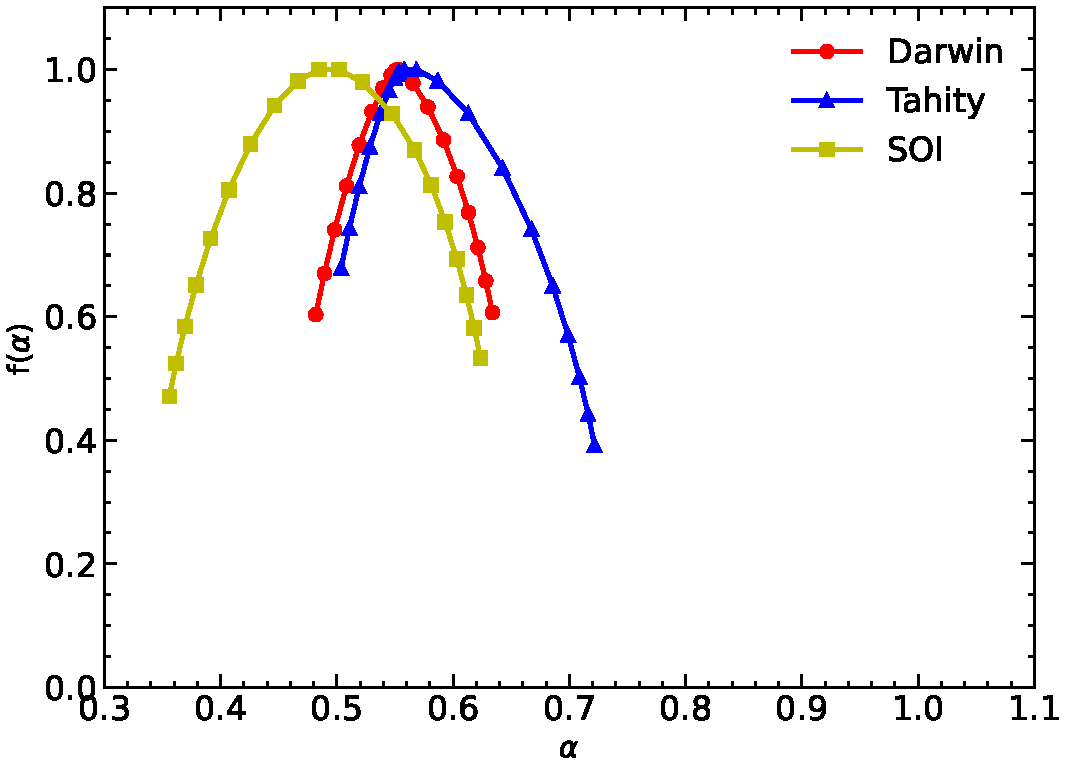
\includegraphics[width=.6\textwidth]{spectrum_shuffle.pdf}} 
\caption{Multifractal spectra for the shuffled series}
\label{fig:spectrum_shuffle}
\end{figure}

\begin{figure}
\centering{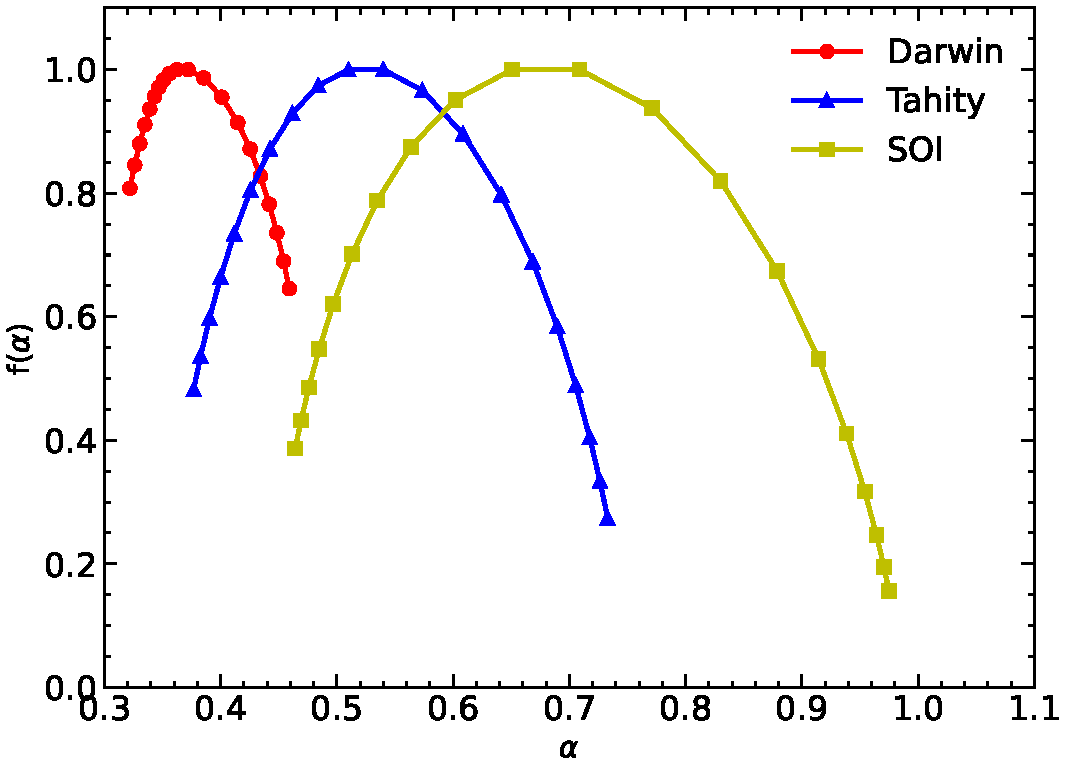
\includegraphics[width=.6\textwidth]{spectrum_surro.pdf}} 
\caption{Multifractal spectra for the surrogated series}
\label{fig:spectrum_surrogate}
\end{figure}

Comparing the two figures we can see that the width of the spectrum of the surrogate data is larger than that of the shuffled ones. This allows us to deduce that long-term correlations play an important role in the multifractality of the data. This is confirmed by the analysis of the absolute value of the differences of the exponent H for original and shuffled data ($\lvert H_{corr}(q)\rvert$) and for original and surrogate data ($\lvert H_{pdf}(q)\rvert$). As we can see in figs. \ref{fig:h-hshuff} and \ref{fig:h-hsurr} $\lvert H_{corr}(q)\rvert > \lvert H_{pdf}(q)\rvert$. This means that the effect of long-range correlations is larger than the broad probability density function. However, non-zero values of $\lvert H_{corr}(q)\rvert$ and $\lvert H_{pdf}(q)\rvert$ indicate that both influence the mutifractality.


\begin{figure}
\centering{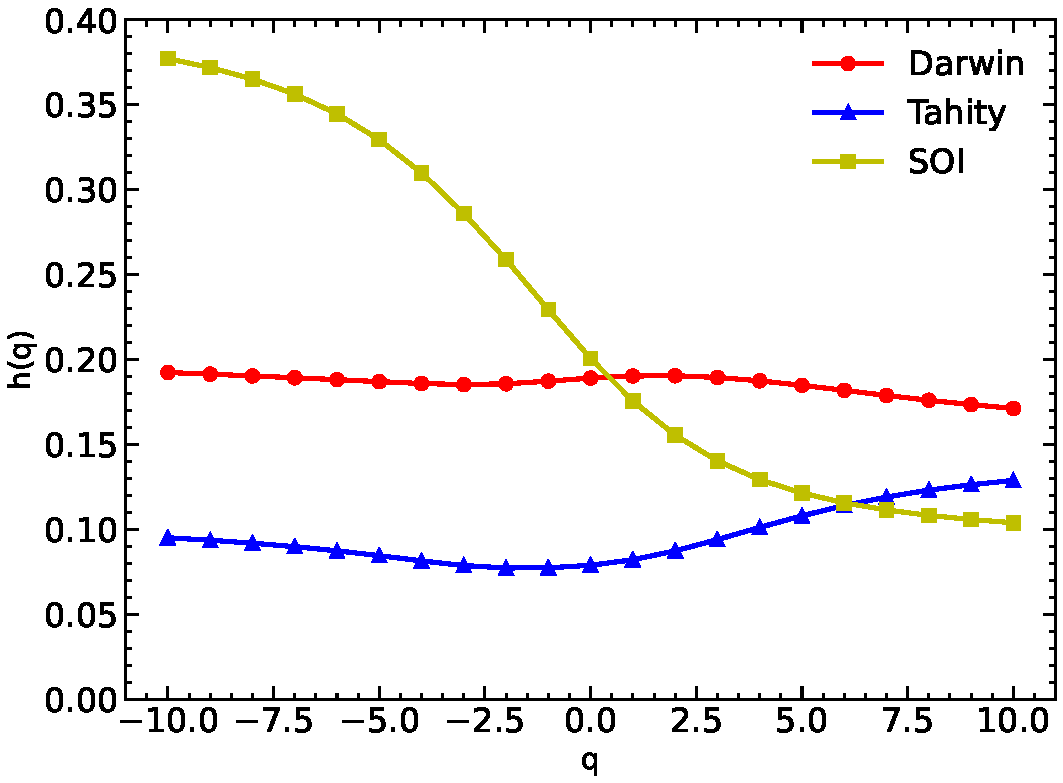
\includegraphics[width=.6\textwidth]{H-Hshuff.pdf}} 
\caption{Multifractal spectra for the shuffled series}
\label{fig:h-hshuff}
\end{figure}

\begin{figure}
\centering{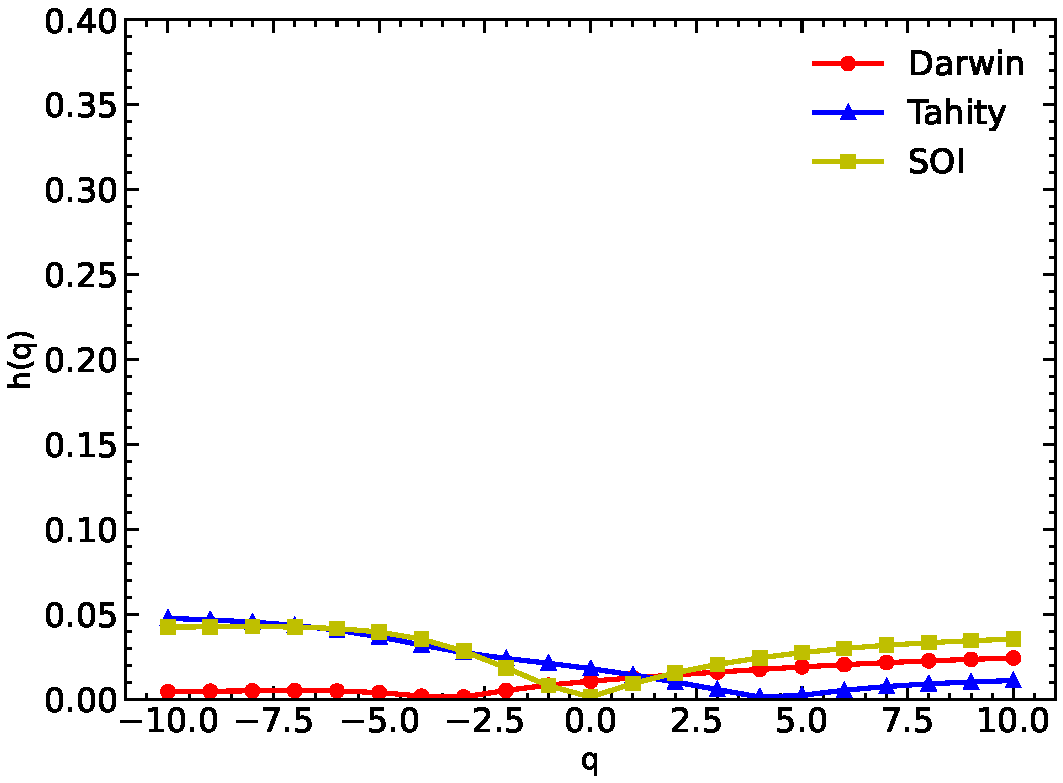
\includegraphics[width=.6\textwidth]{H-Hsurr.pdf}} 
\caption{Multifractal spectra for the surrogated series}
\label{fig:h-hsurr}
\end{figure}


In summary the analyisis performed shows that the mean source of multifractality is the correlation of the values of the series.



\subsection{DCCA}
\label{results_dcca}

We continued our analysis by applying the DCCA method described in the previous section. The DCCA was applied to study the correlation between the time series corresponding to the Darwin and Tahity stations and those corresponding to  each station and the SOI. In order to estimate the level of cross correlation between the series the coefficients $\rho_{DCCA}$ were calculated for each pair of series. The results are shown in figs. \ref{fig:rho_stations} to \ref{fig:rho_tah_soi}.

\begin{figure}
\centering{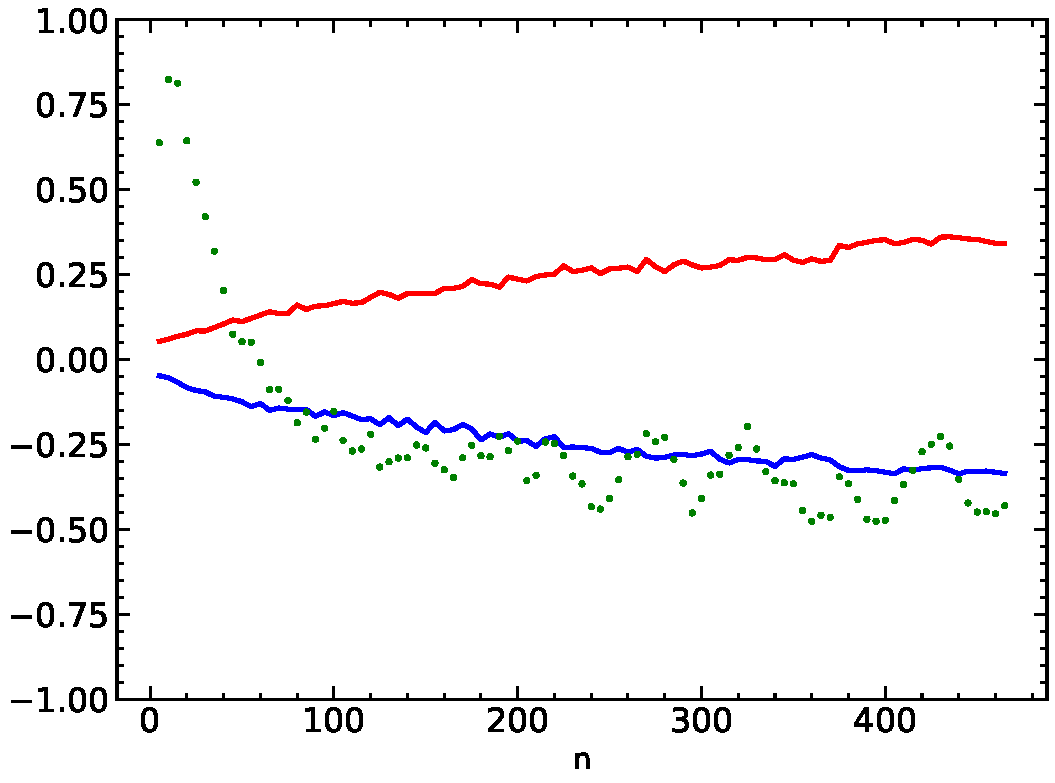
\includegraphics[width=.6\textwidth]{rhoDCCA_stations.pdf}} 
\caption{DCCA cross-correlation coefficient between the two stations (points). The lines corresponds to the 95\% confidence intervals levesl for test of absence of correlation.}
\label{fig:rho_stations}
\end{figure}

\begin{figure}
\centering{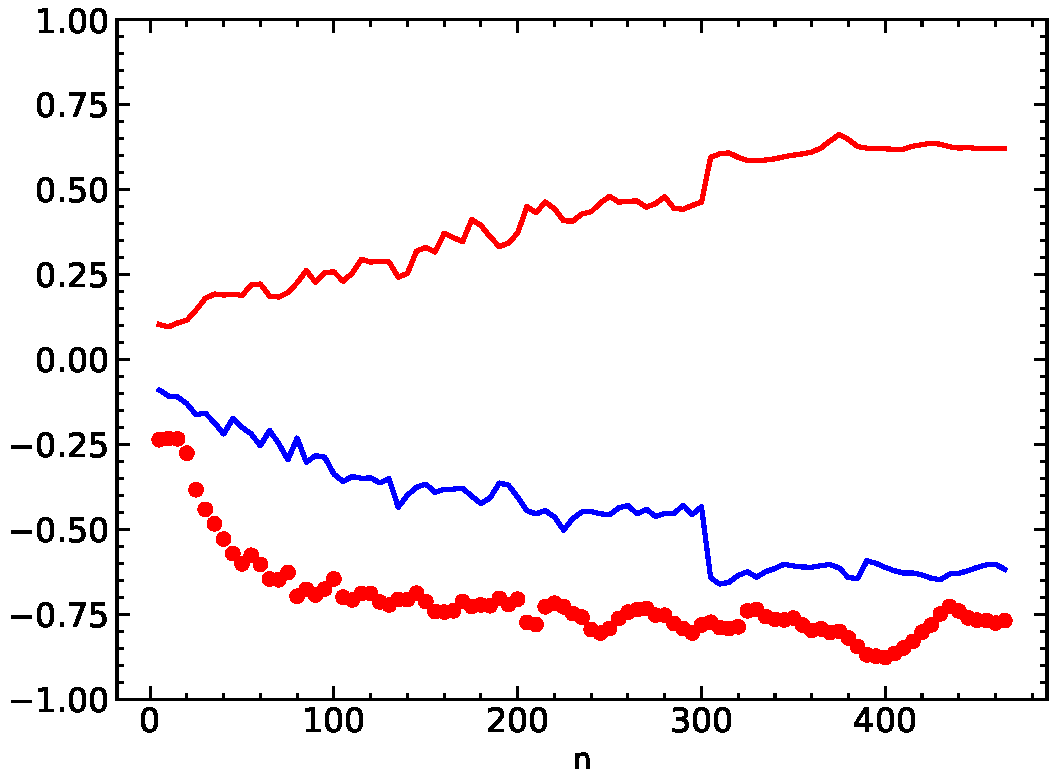
\includegraphics[width=.6\textwidth]{rhoDCCA_dar_soi.pdf}} 
\caption{DCCA cross-correlation coefficient between the SOI index and the Darwin station (points). The lines corresponds to the 95\% confidence intervals levesl for test of absence of correlation.}
\label{fig:rho_dar_soi}
\end{figure}

\begin{figure}
\centering{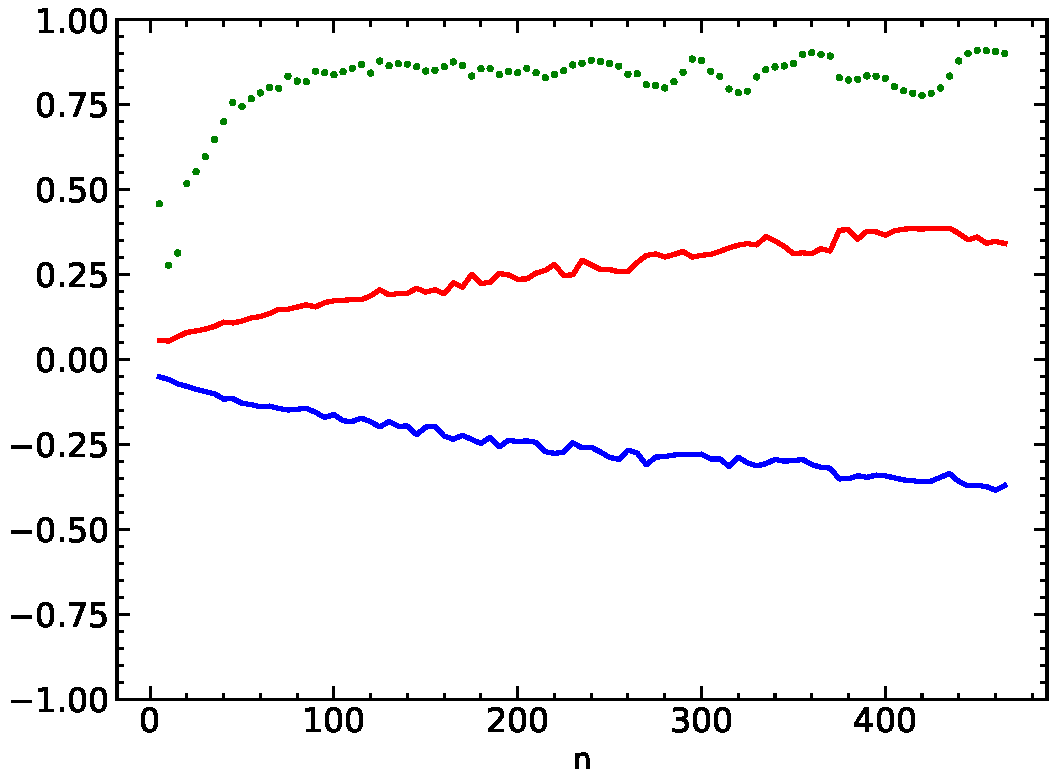
\includegraphics[width=.6\textwidth]{rhoDCCA_tah_soi.pdf}} 
\caption{DCCA cross-correlation coefficient between the SOI index and the Tahity station (points). The lines corresponds to the 95\% confidence intervals levesl for test of absence of correlation. }
\label{fig:rho_tah_soi}
\end{figure}

In the figures We can see that the cross-correlations coefficients tend to stabilize from values of n around 100. It can also be observed that the values of the coefficients are outside the region limited by the confidence intervals, which indicates the the existence of significant cross-correlated behaviors. Generally, we can conclude that the cross-correlations are significant, especially for the correlations between the stations and the SOI index.

\subsection{MF-DCCA}
\label{results_mfdcca}

Finally we apply the MF-DCCA method to analyze the multifractal properties of the bivariate time series. Fig. \ref{fig:mfdcca_H} shows the $q$ dependence of the generalized Hurst exponent. It can be seen from this figure that the value of the Hurst exponent decreases with the increases of $q$. This behavior is more accentuated in the curves that correspond to the pairs between the series of stations and the SOI. In fact, in the case of the $H(q)$ for Darwin-Tahity stations, the variation is much less than the previous ones. The fact that $H
(q)$ is significantly not a constant also reveal that multifractal properties characterize the former pairs. The values of $H(q)$ for $q < 0$ are larger than those for $q > 0$, indicating a more persistent cross-correlation behavior of
small fluctuations compared to large fluctuations. The high value of $H(q)$ is presented by the pair Tahity-SOI.

Also, we observe that for the pairs Darwin-SOI and Tahity-SOI, the values inherent to $q = 2$, the cross-correlation Generalized Hurst exponent are larger than $0.5$. It means that these pairs present persistence behaviour. The fact that the value for $H(2 )$ is always less than $0.5$ in the case of the Darwin-Tahity shows that there is an anti-persistent relationship between these series.

\begin{figure}
\centering{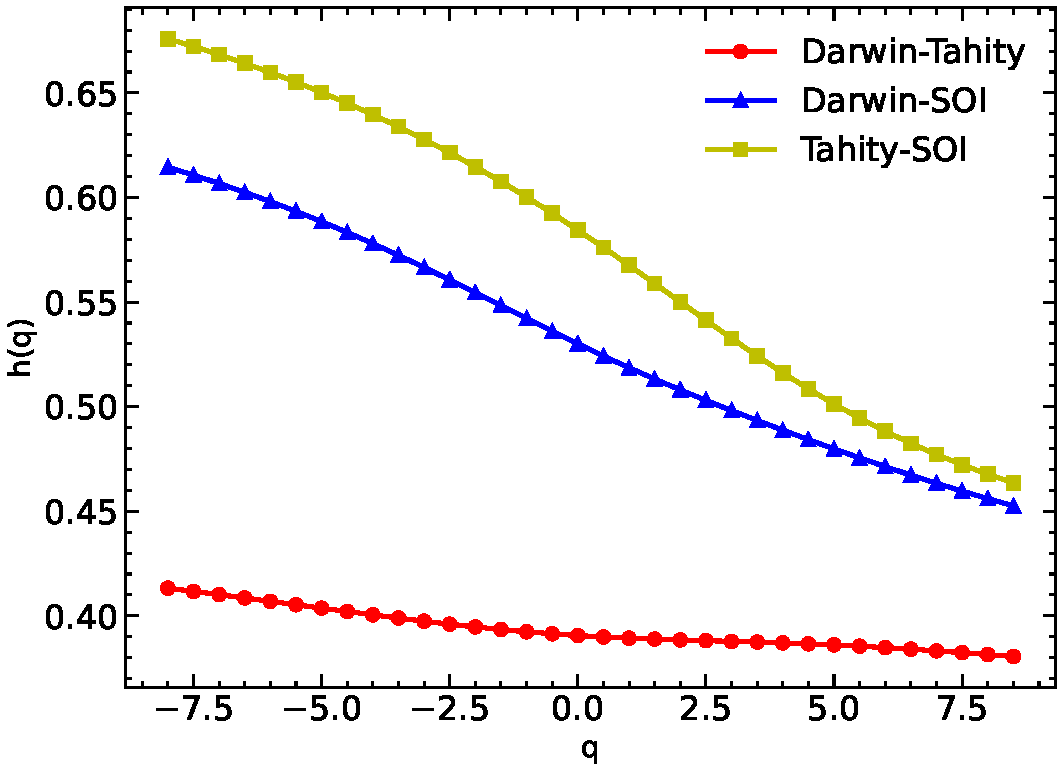
\includegraphics[width=.6\textwidth]{mfdcca_H.pdf}} 
\caption{$q$ dependence of the generalized Hurst exponent}
\label{fig:mfdcca_H}
\end{figure}

\begin{figure}
\centering{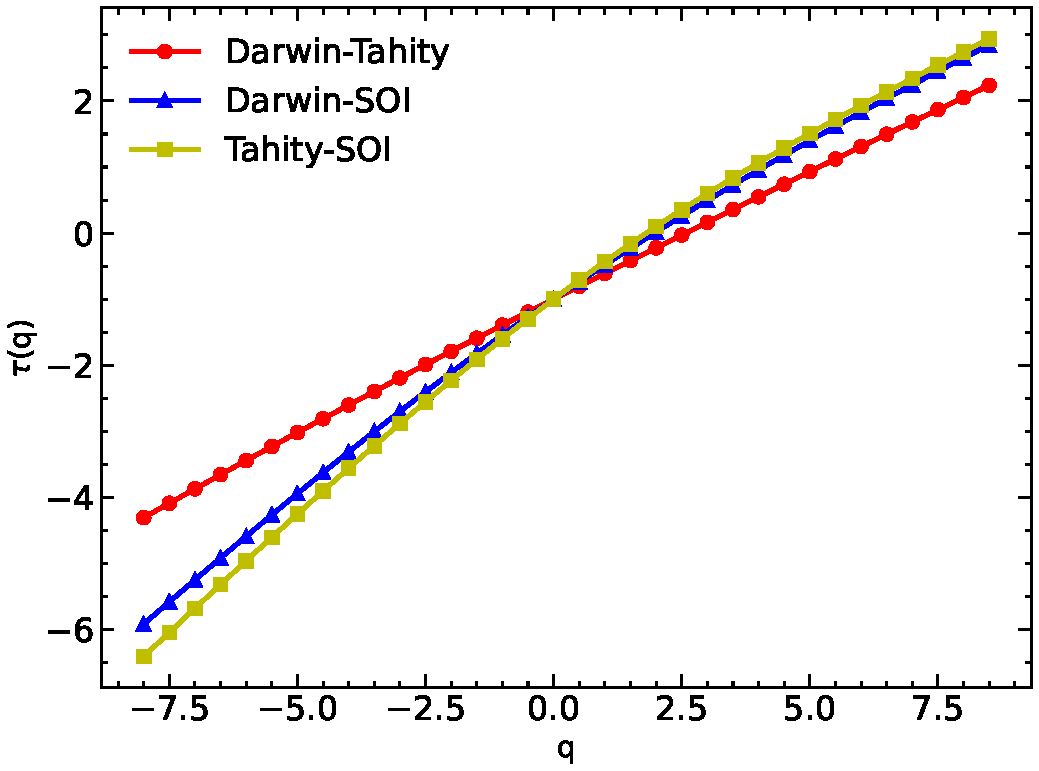
\includegraphics[width=.6\textwidth]{mfdcca_tau.pdf}} 
\caption{Plots of $\tau(q)$ vs $q$}
\label{fig:mfdcca_tau}
\end{figure}

\begin{figure}
\centering{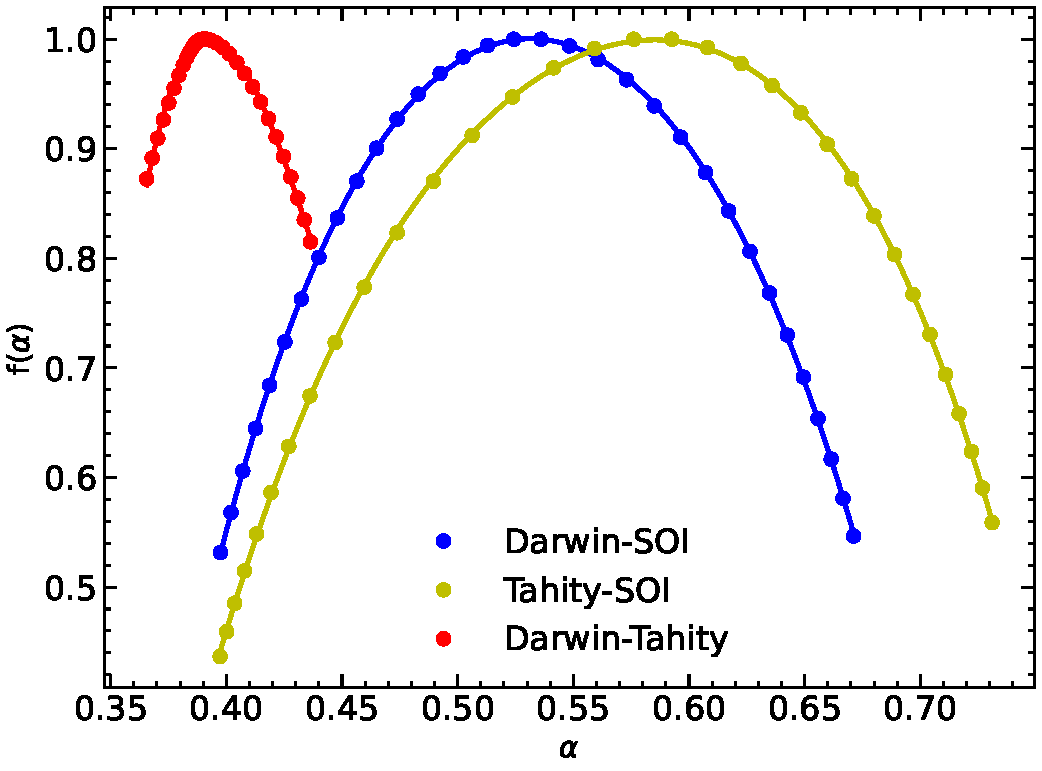
\includegraphics[width=.6\textwidth]{mfdcca_interp_spec.pdf}} 
\caption{Multifractal spectra for the studied series}
\label{fig:mfdcca_spectrum}
\end{figure}

Fig. \ref{fig:mfdcca_tau} displays the $\tau(q)$ vs $q$ plots for each pair of series. The concavity of the function $\tau(q)$ for the pairs between the stations and the SOI show us the nonlinearly dependent of the scaling function on $q$. This behaviour gives evidence of multifractality in the Darwin-SOI and Tahity-SOI pairs. On the contrary, the function $\tau(q)$ is almost linear for the Darwin-Tahity case confirming what we was seen in the plot of $H(q)$.

Finally, fig. \ref{fig:mfdcca_spectrum} shows the singularity spectrum for the bivarite time series. The width of the spectrum can be used to estimate the level of the multifractality. The widths of the cross-correlation multifractal spectra for the Darwin-SOI and Tahity-SOI bivariate series Darwin-SOI and Tahity-SOI, which imply that there are stronger cross-correlation multifractal features between the SOI and stations series. In Table \ref{tab:mfdcca} we present values of different parameters of the multifractal spectra the parameters obtained from the fit of the plots with a fourth degree polynomial.

\begin{table}[t]
\begin{center}
\begin{tabular}{ c  c  c  c  c  c  c  c }
\hline

   & $\alpha_{min}$  & $\alpha_{max}$ & $\alpha_0$ & $f(\alpha_{min})$ & $f(\alpha_{max})$ & $\omega$& $a_s$ \\ \hline
Darwin-SOI   & 0.40  & 0.67  & 0.53  & 0.53 &  0.55 &  0.27 &  -0.01 \\
Tahity-SOI     & 0.40  & 0.73  & 0.59  & 0.44 &  0.56 &  0.33 &  -0.12 \\
Darwin-Tahity     & 0.37  & 0.44  & 0.39  & 0.87 &  0.82 &  0.07 &  0.06 \\
\hline
\end{tabular}
\caption{Characteristics of the multifractal spectrum of the cross correlation}
\label{tab:mfdcca}
\end{center}
\end{table}

The large values of $\alpha_0$, the wider range of fractal exponents and the right-skewed shape that the curves of Darwin-SOI and Tahity-SOI presents,  may be considered a sign of the presence of more complex behaviors in the cross-correlations than the one presented by the Darwin-Tahity time series. The left-sided asymmetry corresponds to a multifractality on the level of larger fluctuations
.
In short, our analysis shows that the time series corresponding to the correlations between the SOI and the stations series have features of multifractality.

\section{Conclusions}
\label{sec:conclusions}

In this paper we use the Detrended Fluctuation Analysis (DFA) method and a multifractal extension of it (MFDFA) to investigate the monofractal and multifractal properties of the the time series of pressure at the sea leavel generated by the Darwin and Tahiti stations. Also we applies these methods to de SOI index. We found evidence of multifractality in the cases of the Tahity and SOI indices. By analyzing the behaviour of the surrogate and shuffle series we show that the main source of multifractality are the long-range correlations. It is interesting to highlight the strong multifractal behavior of the series corresponding to the Tahity station compared to the almost null of the Darwin station series.

We also investigate the cross-correlations between Darwin-Taihty, Darwin-SOI and Tahity-SOI pairs of data by means of the DCCA and MF-DCCA methods. As expected the application of the DCCA method revealed the existence of a significant cross-correlated behavior in the cases of Darwin-SOI and Tahity-SOI series. Finally we apply the MF-DCCA method to analyze the multifractal properties of the cross-correlations. The results obtained through the MF-DCCA method imply that multifractality exists in the cross-relations between the SOI and the Darwin and Tahity stations.

 
\begin{thebibliography}{99}

\bibitem{Dijkstra} \textsc{H. A. Dijkstra},
\textit{Nonlinear Physical Oceanography: A Dynamical
Systems Approach to the Large Scale Ocean Circulation and
El Ni\~no}, Springer Science, New York, 2005.

\bibitem{Sarachik} \textsc{E. S. Sarachik and M. A. Cane},
\textit{The El Ni\~no-Southern Oscillation
Phenomenon}, Cambridge University Press, Cambridge, UK, 2010.

\bibitem{Philander} \textsc{S.G. Philander},
\textit{El Ni\~no, La Ni\~na and the Southern Oscillation},
 Academic Press, San Diego, 1990.

\bibitem{Walker} \textsc{Walker, G.}
\textit{World weather}
\textit{Quarterly Journal of the Royal Meteorological Society}, \textbf{8}, 54, 79-87,1928

\bibitem{Maruyama_1} Maruyama, F. (2019) Relationship between the Atmospheric CO2 and Climate Indices by Wavelet-Based Multifractal Analysis. Journal of Geoscience and Environment Protection, 7, 38-51.

\bibitem{Maruyama_2} Maruyama, F. (2019) Influence of the Atlantic Multidecadal Oscillation and the Pacific Decadal Oscillation on Global Temperature by Wavelet-Based Multifractal Analysis. Journal of Geoscience and Environment Protection, 7, 105-117



%%%%%%%%%%%%%%%%%%%%%%%%%%%%%%%%%%%%%%%%%%%%%%%%%55

\bibitem{Kantelhardt}
Kantelhardt, J.W.; Zschiegner, S.A.; Koscielny-Bunde, E.; Havlin, S.; Bunde, A.; Stanley, H. Multifractal detrended fluctuation analysis of nonstationary time series. {\em Phys. A Stat. Mech. Appl.} {\bf 2002}, {\em 316}, 87--114.
% Reference 2

\bibitem{Peng}
Peng, C.-K.; Buldyrev, S.; Havlin, S.; Simons, M.; Stanley, H.E.; Goldberger, A.L. Mosaic organization of DNA nucleotides. {\em Phys. Rev. E} {\bf 1994}, {\em 49}, 1685--1689
% Reference 3
\bibitem{dcca}Podobnik, B.; Stanley, H.E. Detrended cross-correlation analysis: A new method for analyzing two nonstationary time series. {\em Phys. Rev. Lett.} {\bf 2008}, {\em 100}, 084102.
% Reference 4
\bibitem{dfa}Peng, C.K.; Buldyrev, S.V.; Havlin, S.; Simons, M.; Stanley, H.E.; Goldberger, A.L. Mosaic organization of DNA nucleotides. {\em Phys. Rev. E} {\bf 1994}, {\em 49}, 1685--1689.
% Reference 5
\bibitem{Wang}
Wang, F.; Fan, Q.; Stanley, H. Multiscale multifractal detrended-fluctuation analysis of two-dimensional surfaces. {\em Phys. Rev. E} {\bf 2016}, {\em 93}, 042213.
% Reference 6
\bibitem{Liao}
Wang, F.; Liao, G.; Li, J.H.; Li, X.C.; Zhou, T.J. Multifractal detrended fluctuation analysis for clustering structures of electricity price periods. {\em Physical A Stat. Mech. Appl.} {\bf 2013}, {\em 392}, 5723–-5734.
% Reference 7
\bibitem{Igbawua}
Igbawua, T.; Zhang, J.; Yao, F.; Ali, S. Long Range Correlation in Vegetation Over West Africa from 1982 to 2011. {\em IEEE Access} {\bf 2019}, {\em 7}, 119151–-119165
% Reference 8
\bibitem{Takaishi}
Takaishi, T. Statistical properties and multifractality of Bitcoin. {\em Phys. A Stat. Mech. Its Appl.} {\bf 2018}, {\em 506}, 507–-519.
% Reference 9
\bibitem{Kalamaras}
Kalamaras, N.; Philippopoulos, K.; Deligiorgi, D.; Tzanis, C.G.; Karvounis, G. Multifractal scaling properties of daily air temperature time series. {\em Chaos Solitons Fractals} {\bf 2017}, {\em 98}, 38–-43.
% Reference 10
\bibitem{Podobnik}
Podobnik, B.; Stanley, H. E. . Detrended Cross-Correlation Analysis: A New Method for Analyzing Two Nonstationary Time Series. {\em Phys. Rev. Lett.} {\bf 2008} {\em 100} 1–-11.
% Reference 11
\bibitem {Zhou}
 Zhou,Wei-Xing. Multifractal detrended cross-correlation analysis for two nonstationary signals. {\em Phys. Rev. E} {\bf 2008}{\em 77}, 066211.
% Reference 12
\bibitem{sube}
Datos Abiertos del Ministerio de Transporte. Available online: https://archivos-datos.transporte.gob.ar/upload/Sube/total-usuarios-por-dia.csv
% Reference 13
\bibitem{jh_url}
JHU CSSE COVID-19 Data. Available online: https://github.com/CSSEGISandData/COVID-19.
% Reference 14
\bibitem{jh_journal}
Dong E., Du H., Gardner L., An interactive web-based dashboard to track COVID-19 in real time. {\em Lancet Inf. Dis.} {\bf 2020}, {\em 5}, 533--534.
% Reference 15
\bibitem{Kantelhardt_2}
Kantelhardt, J.W.; Koscielny-Bunde, E.; Rybski, D.; Braun, P.; Bunde, A.; Havlin, S. Long-term persistence and multifractality of precipitation and river runoff records. {\em J. Geophys. Res. Atmos.} {\bf 2006}, {\em 111}, D1. 
% Reference 16
\bibitem{Zhang}
Zhang, Q.; Xu, C.-Y.; Yu, Z.; Liu, C.-L.; Chen, Y.-D. Multifractal analysis of streamflow records of the East river basin (Pearl river), China. {\em Phys. A Stat. Mech. Its Appl.} {\bf 2009}, {\em 388}, 927–-934.
% Reference 17
\bibitem{Dickey_1}
Dickey, D.A.; Fuller, W.A. Distribution of the Estimators for Autoregressive Time Series with a Unit Root. {\em J. Am. Stat. Assoc.} {\bf 1979}, {\em 74}, 427–-431.
% Reference 18
\bibitem{Dickey_2}
Dickey, D.A.; Fuller, W.A. Likelihood Ratio Statistics for Autoregressive Time Series with a Unit Root. {\em Econom. J. Econom. Soc.} {\bf 1981}, {\em 49}, 1057–1072.
% Reference 18
\bibitem{Theiler}
Theiler J, Galdrikian B, Longtin A, Eubank S, Farmer D. J. Using surrogate data to detect nonlinearity in time series. In: {\em Nonlinear modeling and forecasting}. Casdagli M., Eubank S.(eds) Addison-Wesley, Redwood City, CA, 1992, 163--188
\bibitem{Zebende}Zebende G, da Silva P A and Filho A M 2011 Study of crosscorrelation
in a self-affine time series of taxi accidents.Physica A 390 1677–83
 
\bibitem{Peng_3} \textsc{C.K. Peng, S.V. Buldyrev, S. Havlin, M. Simons, H.E. Stanley, A.L. Goldberger},\textit{Mosaic organization of nucleotides.} Phys. Rev. E, 49 (1994), p. 1685

\bibitem{Huang} \textsc{Huang, Norden E.  and Shen, Zheng  and Long, Steven R.  and Wu, Manli C.  and Shih, Hsing H.  and Zheng, Quanan  and Yen, Nai-Chyuan  and Tung, Chi Chao  and Liu, Henry H.}, \textit{The empirical mode decomposition and the Hilbert spectrum for nonlinear and non-stationary time series analysis}, \textit{Proceedings of the Royal Society of London. Series A: Mathematical, Physical and Engineering Sciences}, 454, 1971, 903-995, 1998
\bibitem{Buldyrev_2}S.V. Buldyrev, N.V. Dokholyan, A.L. Goldberger, S. Havlin, C.-K. Peng, H.E. Stanley, G.M. Viswanathan
Analysis of DNA sequences using methods of statistical physics.
Physica A, 249 (1998), p. 430
\bibitem{Buldyrev_3}S.V. Buldyrev, A.L. Goldberger, S. Havlin, R.N. Mantegna, M.E. Matsa, C.-K. Peng, M. Simons, H.E. Stanley
Long-range correlation properties of coding and noncoding DNA sequences: GenBank analysis
Phys. Rev. E, 51 (1995), p. 5084
\bibitem{Peng_2}C.-K. Peng, J. Mietus, J.M. Hausdorff, S. Havlin, H.E. Stanley, A.L. Goldberger
Long-Range anticorrelations and non-Gaussian behavior of the heartbeat
Phys. Rev. Lett., 70 (1993), p. 1343
\bibitem{Viswanathan}G.M. Viswanathan, C.-K. Peng, H.E. Stanley, A.L. Goldberger
Deviations from uniform power law scaling in nonstationary time series.
Phys. Rev. E, 55 (1997), p. 845
\bibitem{Echeverria}J. C. Echeverr\'ia
Interpretation of heart rate variability via detendred fluctuation analysis.
Chaos: An Interdisciplinary Journal of Nonlinear Science 13 (2003), p. 467
\bibitem{Cizeau}P. Cizeau, Y.H. Liu, M. Meyer, C.-K. Peng, H.E. Stanley
Volatility distribution in the S\&P500 stock index.
Physica A, 245 (1997), p. 441
\bibitem{Ausloos}M. Ausloos, K. Ivanova
Introducing \textit{False} EUR and \textit{False} EUR exchange rates.
Physica A, 286 (2000), p. 353
\bibitem{Jaroszewicz}Jaroszewicz S., Mariani M., Ferraro M.
Long correlations and truncated Levy walks applied to the study Latin-American market indices
Physica A, 355 (2005), pp. 461-474
\bibitem{Mariani}Mariani M., Florescu I., Varela M., Ncheuguima E.
Long correlations and Levy models applied to the study of memory effects in high frequency (tick) data
Physica A, 388 (2009), pp. 1659-1664
\bibitem{Ribeiro}R. A. Ribeiro, M. V. M. Mata, L. S. Lucena, U. L. Fulco, and G. Corso
Spatial analysis of oil reservoirs using detendred fluctuation analysis of geophysical data.
Nonlin. Processes Geophys., 21, 1043–1049, 2014

\end{thebibliography}0

\end{document}
